\documentclass[../../Aurora C# unofficial manual.tex]{subfiles}

\begin{document}
	\section{Adding planets, comets and asteroid belts}\label{5_adding_planets_comets_asteroid}
	Original post can be found
	\href{http://aurora2.pentarch.org/index.php?topic=8495.msg118767#msg118767}{here}.
	\\\\
	
	Below is the form for adding all new system bodies except for additional moons. You choose a system body from the drop down, which includes Terrestrial, Dwarf Planet, Gas Giant, Superjovian, Comet and Asteroid. Each body type has a distance parameter plus one or more other additional options.
	\begin{itemize}
		\item For terrestrial and dwarf planets you have a toggle for automatic moon generation and can choose a specific or random number of moons.
		\item For gas giants and superjovians, you have the above moon options plus similar options for Trojan asteroids (on/off, random/specific).
		\item For comets, you choose the starting distance and maximum distance.
		\item For asteroid belts, you can choose a random or specific number of asteroids and the specific or random width of the belt (how far an asteroid can be generated from the centre of the belt).
	\end{itemize}
	
	Once the planet parameters are selected, press OK and the new body or bodies will appear in the System View. You can select them and use Modify Body to customise if desired.
	
	The various zones shown at the top affect how Aurora determines parameters such as atmosphere, hydrosphere, mineral deposits, albedo, density, number of moons, total mass of asteroid belts and a variety of other factors. There is far too much detail to list, but generally bodies in the life zone will have better conditions and mineral deposits, followed in decreasing order by Inner, Outer and Extreme. These zones also exist in VB6. Of course, those factors only affect initial generation so you can override that by directly modifying a body post-creation.
	\begin{figure}[H]
		\centering
		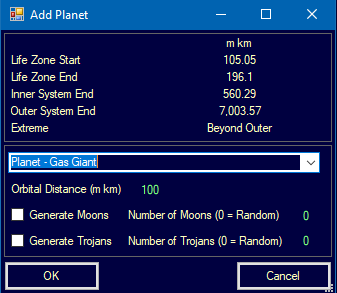
\includegraphics[width=0.5\linewidth]{images/AddPlanet}
		\caption[Add Planet Example]{Add Planet Example}
		\label{fig:addplanet}
	\end{figure}
\end{document}